\documentclass[12pt]{article}

%-------Packages---------
\usepackage{amssymb,amsfonts}
\usepackage{enumerate}
\usepackage[margin=0.75in]{geometry}
\usepackage{rotating}
\usepackage{amsthm}

\newtheorem{theorem}{Theorem}[section]
\newtheorem{lemma}[theorem]{Lemma}
\newtheorem{proposition}[theorem]{Proposition}
\newtheorem{corollary}[theorem]{Corollary}
\newenvironment{definition}[1][Definition]{\begin{trivlist}
\item[\hskip \labelsep {\bfseries #1}]}{\end{trivlist}}

%--------Meta Data: Fill in your info------
\title{Order Preserving Encryption Schemes: \\
  Preventing the Leakage of Distribution\\
6.857 Final Paper \\
Hrishikesh Joshi, Max Kolysh, Mari Miyachi, John Wang}

\begin{document}

\maketitle

\section{Distribution Confidentiality Scheme}

In order to solve the problem of leaking the distribution of the plaintext values, we have developed the Distribution Confidentiality Scheme (DCS). This scheme uses Raluca et al (2013)'s original mOPE scheme, but adds an additional layer of security.

In essence, the DCS scheme adds random bits to the end of a plaintext so that the ciphertext values are randomized. This will prevent the server from being able to identify the number of times a repeated plaintext value is inserted.

\subsection{Description of DCS}

This section will give a formal description of DCS. We will first describe the basic version of the scheme, then we will augment it so that decimal numbers can be represented as well.

In the basic version of the scheme, let us assume that we want to encrypt some plaintext value $x \in \mathrm{Z}$ and send it to the server like in Raluca et al (2013)'s mOPE scheme. For DCS, there is an additional parameter $\rho$ which will govern the probability with which the server sees a repeated value. We will generate a random value $r \in [0,1)$ which contains $\rho$ bits, denoted $r_{\rho}$, and append it to the end of $x$. The resulting value $x' = x + r_{\rho}$ will be encrypted with DET. Raluca et al (2013)'s mOPE scheme will work the same as before, but now acting on $x'$.

Inserting in this scheme is simple, since nothing really has to be changed from Raluca et al (2013)'s mOPE scheme. The client will take the value $x$ to insert, create $x'$, then encrypt $x'$ to obtain a ciphertext. Inserting this ciphertext will involve moving down the server's binary search tree. The insertion process is started by the client acquiring the root node. The client then checks to see if $x'$ is larger or smaller than the root's decrypted value. This informs the client as to the direction in which it should move. Once it arrives at a leaf node, the client will insert the new ciphertext in the correct direction.

\begin{figure}
%\lstset{language=Python}
%\begin{lstlisting}
%  TODO: Insert the insertion pseudocode here.
%\end{lstlisting}
%\caption{Pseudocode for the Insertion Algorithm}
%\label{insertion_figure}
\end{figure}

Querying, however, gets more difficult, and the next section will discuss how the client can query for some value $y$.

\subsection{Querying Under DCS}

  To query for some value $y$, we must actually perform a range query, since any value $y$ will be encrypted with a plaintext $y + r$ where $r \in [0,1)$. This means, the encrypted plaintext of $y$ can therefore take in the range $[y, y + 1)$. Thus, to query for the value $y$, we must perform a range query on any values in the range $[y, y+1)$.

  Performing this range query on the binary search tree can be done by searching for $y$ and $y+1$ individually. Once we have found $y$ and $y+1$, then we can move up the tree until we find the least common ancestor between the nodes of $y$ and $y+1$. The subtree rooted at the least common ancestor will contain all possible values in the range $[y, y+1)$.

  \begin{lemma}
    The subtree rooted at the least common ancestor of $y$ and $y+1$ in a binary search tree contains all values $x \in [y, y+1)$.
  \end{lemma}
  \begin{proof}
    Let us examine some value $x \in [y, y+1)$, and call the $l$ the least common ancestor of $y$ and $y+1$.

    Now suppose $x$ is not in the subtree rooted at $l$. This means that $x$ must either be smaller than the left-most node in the subtree rooted at $l$ or greater than the right-most node in the subtree (assuming that no nodes are have repeated values which occurs with high probability because of the random bits $r$ appended to each plaintext). However, we know that the left-most node in the subtree rooted at $l$ must be smaller than $y$ and the right-most node in the subtree must be greater than $y+1$. This is true because both $y$ and $y+1$ are nodes in the subtree.

    This is a contradiction, however, because we assumed $x \in [y, y+1)$, which shows that the subtree contains all values $x \in [y, y+1)$.
  \end{proof}

This lemma instructs us on how to find all values $x \in [y, y+1)$. As we move up the binary search tree to parents of $y$, we check the right subtree of the parent looking for all values in $[y, y+1)$. We do this as we continue upwards for all successive parent nodes. For the node at $y+1$, we check the left subtree of all parents for values in $[y, y+1)$. We continue this process until the parent of the $y$ node meets the parent of the $y+1$ node. This process will find all values in $[y, y+1)$, because as we have shown, all values in the interval are inside the subtree.

  This process is correct because we continue checking subtrees until we find the least common ancestor for the parents of both the $y$ and the $y+1$ nodes. The runtime of this is just $\log(n) + K$ where $K$ is the number of values in the range $[y, y+1)$.

  \subsection{Range Queries Under DCS}

  To perform range queries under the DCS scheme, one simply needs to perform a range query on the underlying binary search tree. If one attempts to query for values $x \in [y, z]$, then we simply perform a range query for the underlying plaintexts in the binary search tree in the range $[y, z+1)$. We use the same range query mechanism as in the previous section, making sure to only output values that are inside in the interval $[y, z+1)$.

\section{Indistinguishability Under Chosen Plaintext Distribution Attack (IND-CPDA)}

This security definition consists of two phases of interaction between the adversary and the challenger.

In phase I:
\begin{itemize}
  \item Client generates $SK \leftarrow KeyGen(1^\kappa)$ based on security parameter $\kappa$.
  \item Adversary may perform encryptions and other operations in time $poly(\kappa)$.
\end{itemize}

In phase II, the client and server engage in $poly(\kappa)$ rounds of interaction in which the adversary is adaptive. In each round $i$:
\begin{itemize}
  \item Adversary sends sequences $V_i^0, V_i^1 \in D^{\lambda}$ to the client each of size $\lambda$, where $\lambda$ is a fixed value, and $V_i = \{ v_{ij} \}_i^{\lambda}$ where $v_{ij}$ is the $j$th value chosen for round $i$.
  \item The client leads the interaction for the encryption algorithm on inputs $SK$ and $V_i^b$ with the server, with the adversary observing all the state at the server.
\end{itemize}

In phase III:
\begin{itemize}
  \item Adversary obtains $poly(\lambda, \kappa)$ time to compute.
  \item Adversary outputs $b'$ as its guess for $b$. 
\end{itemize}

The adversary shall win the game if its guess is correct $b' = b$ and the sets have the same order relations (namely that $v_{ij}^0 < v_{ik}^0 \Leftrightarrow v_{ij}^1 < v_{ik}^1$).

\begin{definition}
  The adversary's advantage is the difference $|Pr[\textrm{win}^{Adv, \kappa, \lambda}] - 1/2|$.
\end{definition}

\begin{definition}
  IND-CPDA. A mOPE scheme is IND-CPDA secure if for all adversaries and all sufficiently large $\kappa$ and $\lambda$, the adversary's advantage is negligible, i.e. that $Pr[\textrm{win}^{Adv, \kappa, \lambda}] \leq 1/2 + \textrm{negl}(\kappa, \lambda)$.
\end{definition}

\subsection{Security of DCS}

\begin{theorem}
  DCS is IND-CPDA secure 
\end{theorem}
\begin{proof}
We shall show that encrypting $v = \{V_1, V_2, \ldots, V_{\kappa} \}$ and $w = \{W_1, W_2, \ldots, W_{\kappa}\}$ is information-theoretically the same, where $V_i, W_i$ are sequences of size $\lambda$.

We will show this by induction on the number of repeated elements in either $V_i$ or $W_i$. We shall first consider the base case when there are no repeated elements in $V_i$ or in $W_i$, so that all the elements in $V_i$ are distinct, as well as the elements in $W_i$. In this case, the sequence $v$ can be broken down into $\kappa$ sequences of all distinct elements. This has a clear bijection to a sequence of elements $v_{ij}$ of length $\kappa \lambda$, for $i \in \{1, 2, \ldots, \kappa\}$ and $j \in \{1, 2, \ldots, \lambda \}$. Winning this game then becomes equivalent to winning the IND-OCPA security game, since one can think of each $v_{ij}$ and $w_{ij}$ pair as a set of values that the adversary provides the client in each round $i$. Popa et al (2013) shows that their scheme, which is equivalent to the Distribution Confidentiality Scheme when there are no reptitions, is IND-OCPA secure. This means that the DCS scheme is IND-CPDA secure when there are no repeated elements.

Now we shall use strong induction and assume that when there are a maximum of $k$ repeated elements in both $V_i$ and $W_i$, the DCS scheme is IND-CPDA secure. To complete the proof, we simply need to show that when there are $k+1$ repeated elements, the DCS scheme is still secure.

Let us compare the sets $V_i$ and $W_i$ with $k+1$ repeated elements to the sets with $k$ repeated elements. In the $k+1$ case, there is one extra reptition with a value that has already appeared, on top of the $k$ repetitions that already exist. Now consider the plaintext $x$ which is repeated. The probability that the OPE encoding of $x$ has already appeared in the sequence of elements in the set $V_i$ or $W_i$ is negligible at $O(2^{-\lambda} \kappa)$. Since the OPE encoding is not repeated by the new value $x$, the number of OPE encoding repetitions is at most $k$. However, we have shown that when there are $k$ repeated elements in the sets $V_i$ and $W_i$, then DCS is IND-CPDA secure by the inductive hypothesis. Since the largest number of repeated encodings in this case is $k$, this is the same situation as when there are $k$ repeated elements in the sets $V_i$ and $W_i$. Therefore, when there are $k+1$ repeated elements, DCS is IND-CPDA secure.

We have therefore shown by induction that DCS is IND-CPDA secure for any number of repeated elements in the sets $V_i$ and $W_i$, which completes the proof that DCS is IND-CPDA secure.
\end{proof}

\section{Random Tiebreaking Order Preserving Encryption (RTOPE)}

  Consider a simple tie-breaking rule on top of Popa et al (2013)'s mOPE scheme. When the client inserts a new ciphertext $c^*$ into the server, the client proceeds normally when the ciphertext $c_i$ returned by the server does not correspond to a plaintext $p_i$ which is equal to $p^* = Dec(SK, c^*)$. However, if $p_i = p^*$, then the client tells the server to move left or right with uniform probability. Note that in this scheme, we will use a randomized encryption scheme which is IND-CCA so that the server cannot tell if two plaintext values are the same.

  To query a ciphertext $c^*$, one needs to make sure to find all possible places where $c^*$ can exist. Thus, whenever the server returns $c_i$ which decrypts to $p_i = p^* = Dec(SK, c^*)$, then one must check both the left and right subtrees of $c_i$ to see if $c^*$ exists. Querying each subtree is done with the  normal Popa et al (2013) process.

  This scheme is a simple extension of Popa et al (2013)'s scheme and handles repeated values. In RTOPE, the server cannot tell how many values are repeated, and what the distribution of repeated values looks like.

  \subsection{Querying Under RTOPE}

  Under RTOPE, there are multiple variations on querying for some value $x$. First is to query for just one ciphertext whose corresponding plaintext is equal to $x$. The second query type is to query for all ciphertexts whose corresponding plaintext is equal to $x$. 

  The first case is easy to handle and can be achieved by using the regular query mechanism used by Popa et al (2013) and returning the first ciphertext found which matches. If there are any ciphertexts which can be decrypted to $x$, then the regular binary search tree mechanism will find at least one, which guarantees that this will correctly return one of these ciphertexts.

  The second case can be handled by a modified query algorithm. To return all ciphertexts decrypting to $x$, we still need to do a regular query for $x$. Upon finding the first $x$, we append this value to our list of results, and we need to query both the right and left subtrees for $x$ again. Doing this recursively until we reach a leaf will guarantee that we will find all possible places where $x$. This gaurantee can be given in the following proposition:

  \begin{proposition}
    Let $T$ be a binary search tree and $x$ be a repeated value in the binary search tree. There exists a subtree $T'$ rooted at $x$ which contains all values $x$ in the tree $T$.
  \end{proposition}
  \begin{proof}

  \end{proof}

  By the above proposition, we can show that as soon as we find the first value of $x$ based on the regular binary search tree query algorithm, then all other values of $x$ will be contained in either the left or right subtree of this node. This implies that we will find all values of $x$ in the tree.

  \subsection{Security of RTOPE}

  RTOPE can be proven to be IND-CPDA, just like the DCS scheme.

  \begin{theorem}
    RTOPE is IND-CPDA secure.
  \end{theorem}
  \begin{proof}
    Like in the security proof for DCS, we shall show that encrypting $v = \{V_1, V_2, \ldots, V_{\kappa} \}$ and $w = \{W_1, W_2, \ldots, W_{\kappa}\}$ is information-theoretically the same, where $V_i, W_i$ are sequences of size $\lambda$. Again, we shall use induction on the number of repeated elements in either $V_i$ or $W_i$. 

    When there are no repeated elements, we can use the same argument we used in the DCS proof. We note that the sequence $\{V_1, V_2, \ldots, V_{\kappa} \}$ has a bijection to a sequence of elements $v_{ij}$ of length $\kappa \lambda$, for $i \in \{1, 2, \ldots, \kappa\}$ and $j \in \{1, 2, \ldots, \lambda \}$. Winning this game then becomes equivalent to winning the IND-OCPA security game, since one can think of each $v_{ij}$ and $w_{ij}$ pair as a set of values that the adversary provides the client in each round $i$. Popa et al (2013) shows that their scheme, which is equivalent to the Distribution Confidentiality Scheme when there are no reptitions, is IND-OCPA secure. Thus, the base case of no repetitions is secure.

    Now, suppose that RTOPE is IND-CPDA secure when there are at most $k$ repetitions across $V_i$ and $W_i$. Now consider a sequence where there are $k+1$ repetitions across $V_i$ and $W_i$ for all $i$. Select two ciphertexts $c_1$ and $c_2$ of some repeated value $x$ and let us consider how it this pair of repetitions is inserted into the tree. Since RTOPE uses an encryption scheme which is IND-CCA for its ciphertexts, the adversary will not be able to tell whether $Dec(SK, c_1) = Dec(SK, c_2)$ with more than $1/2$ probability (by the definition of IND-CCA security). This means that the adversary cannot distinguish $c_1$ and $c_2$ as being repetitions with any advantage. Thus, a sequence of $k+1$ repetitions is information theoretically the same for the adversary as a sequence of $k$ repetitions, which we already know is IND-CPDA secure. Using induction, we have completed the proof.  
  \end{proof}

\section{Relationship Between DCS and RTOPE}

  In this section, we shall propose a notion of equivalence between two OPE schemes.

  \subsection{Structural Expectation Equivalence}

  \emph{Definition:} Two OPE schemes $x,y$ are \emph{Structural Expectation Equivalent} if for each plaintext $p_i$ that scheme $x$ encodes in a sequence of plaintexts $P = \{p_i\}_{i=1}^n$, there exists some bijective mapping $f: \mathrm{Z}_y \to \mathrm{Z}_x$ where $Pr[Encode_x(c_i) = \omega] = Pr[f(Encode_y(c_i)) = \omega]$ for all $\omega \in \mathrm{Z}_x$ where $\mathrm{Z}_x$ is the space of all possible OPE encodings for scheme $x$, $c_i = Enc(SK, p_i)$ is the ciphertext corresponding to $p_i$, and $Encode_x(c_i)$ and $Encode_y(c_i)$ are the functions that obtain the OPE encoding for schemes $x$ and $y$ respectively.

  In other words, for two schemes to be structurally expectation equivalent, there must exist a mapping $f$ from all of the possible OPE encodings from scheme $x$ to scheme $y$, where the probability of obtaining an encoding in $x$ is the same as the probability of obtaining the corresponding encoding in $y$ (based on the mapping). This must be the case for all possible encodings.

  This notion of structural expectation equivalence encompasses a number of useful features. In particular, notice that if $x$ is an OPE encoding scheme which is IND-CPDA secure, and $y$ is structurally expectation equivalent to $x$, then $y$ is also IND-CPDA secure. Due to this notion, it is sufficient to show the structural expectation equivalence of two schemes in order to link the IND-CPDA security of the schemes (the proof of this property is given in the theorem below). Another observation one can make is that the mapping in the structural expectation equivalence definition is bijective. Hence, if $x$ is structurally expectation equivalent to $y$, then $y$ is necessarily structurally expectation equivalent to $x$ because one can simply use $f^{-1}$ as the mapping, which necessarily exists because of $f$ being bijective.

\begin{theorem}
 If two OPE schemes $x,y$ are structurally expectation equivalent, then $x$ is IND-CPDA secure if and only if $y$ is IND-CPDA secure.
\end{theorem}
\begin{proof}
  First, we observe that notion of equivalence is symmetric (since $f$ is a bijective mapping which is invertible), so that without loss of generality, we need only show that if $x$ is IND-CPDA secure, then $y$ is as well. So now we can suppose that $x$ is IND-CPDA secure and $x,y$ are equivalent schemes.

  Since $x$ is IND-CPDA secure, then for any two sequences $v = \{V_1, V_2, \ldots, V_{\kappa}\}$ and $w = \{W_1, W_2, \ldots, W_{\kappa} \}$ that the adversary provides, the adversary cannot correctly distinguish between $v$ and $w$ with non-neglible advantage. Now suppose by contradiction that $y$ is not IND-CPDA secure. Then there exist two sequences $v' = \{V_1', \ldots, V_{\kappa}'\}$ and $w' = \{W_1', \ldots, W_{\kappa}'\}$ of plaintexts that the adversary can provide to the client so that he can distinguish the two sequences with non-neglible advantage in the client-server interaction. This means that the adversary can distinguish the encoding $Encode_y(V_i') = \{Encode_y(V_{ij}' \}_{j=1}^{\lambda}$ for some $i$ from the encoding $Encode_y(W_i') = \{Encode_y(W_{ij}') \}_{j=1}^{\lambda}$.

  This means the adversary can also distinguish the mapping $Encode_x(V_i')$ from the encoding $Encode_x(W_i')$ by applying the bijective mapping $f$ (from the definition of equivalence) to obtain $Encode_x(V_i') = f(Encode_y(V_i'))$ and $Encode_x(W_i') = f(Encode_y(W_i'))$. This is a contradiction because it shows that $x$ is not IND-CPDA secure, which was one of our assumptions. Thus, we see by contradiction that $y$ must be IND-CPDA secure, which proves our result.
\end{proof}

  \subsection{Structural Expectation Equivalence of DCS and RTOPE}

  In this section, we shall investigate whether DCS and RTOPE are structurally expectation equivalent. To do this, we shall first examine some propositions.

\begin{proposition}
  There exists some subtree which contains all the ciphertexts corresponding to a plaintext $x$ in both DCS and RTOPE.
\end{proposition}
\begin{proof}
  This proposition is immediately clear because one can always take the entire tree as the subtree. This works for the cipher text trees stored in both DCS and RTOPE.
\end{proof}

Since a subtree containing all the ciphertexts corresponding to a plaintext $x$ exists, we can now examine properties of this subtree. First, we show that the root of the smallest possible such subtree must be a ciphertext which gets decrypted to $x$.

\begin{proposition}
  The smallest subtree containing all ciphertexts which can be decrypted to some plaintext $x$ is rooted at a ciphertext $c$ such that $x = Dec(SK, c)$ in both DCS and RTOPE.
\end{proposition}
\begin{proof}
  First, we know that a subtree containing all ciphertexts which can be decrypted to $x$ exists, by the proposition we gave above. We therefore also know that a smallest subtree exists because the entire tree is of finite size. Now we shall show that this smallest subtree is rooted at $c$ such that $x = Dec(SK, c)$ for DCS.

  Suppose not, by contradiction. Then some ciphertext $c'$ is at the root such that $x' = Dec(SK, c')$ where $x' \neq x$. Since DCS is normalized to integer plaintexts, we must have $|x' - x| \geq 1$. We know, moreover, that there must be at least one ciphertext $c_l$ in the left subtree of the root and $c_r$ in the right subtree of the root such that $x = Dec(SK, c_l) = Dec(SK, c_r)$. If not, then the subtree we are in is not the smallest subtree containing all ciphertexts which decrypt to $x$ because one can simply take either the right or left subtree (depending on if the left or right subtree does not contain $c_l$ or $c_r$ respectively).

  However, we know that $Dec(SK, c_l) \leq Dec(SK, c') \leq Dec(SK, c_r)$ by the fact that $c_l$ is in the left subtree of $c'$ and that $c_r$ is in the right subtree. This implies that $x \leq x' \leq x$ so that $x' = x$. However, this is a contradiction because we assumed that $x' \neq x$. We have therefore shown that for DCS, the smallest subtree containing all cipertexts decrypting to $x$ must be rooted at a ciphertext decrypting to $x$.

  The proof for RTOPE is similar and we only provide a sketch. If $c'$ is a root which does not decrypt to $x$, then it must be separating a left and right subtree which contain $c_l$ and $c_r$, respectively, which decrypt to $x$. This means that $Dec(SK, c_l) \leq Dec(SK, c') \leq Dec(SK, c_r)$ which means that $x' = x$, which results in a contradiction (just like in the proof for DCS).
\end{proof}

We have seen that the smallest subtree containing a repeated plaintext will be rooted at a ciphertext decrypting to that plaintext. This has a number of interesting applications. For instance, one can examine the series of decisions that are made in the RTOPE scheme by the client by examining this subtree and a smaller subtree in a recursive fashion.

For DCS, one can see that moving left or right from the root element depends on the relative size of the root element with the new element being inserted or queried. For example, if $x$ is the value of a repeated plaintext, then DCS will mutate $p$ into $p + r$ where $r \in [0,1)$ are some random bits. Moving left at the root means that $p_1 < p_r$ where $p_r$ is the root value. This means that $p + r_1 < p + r_r$, which is equivalent to saying $r_1 < r_r$. Thus, moving left at the root is just the probability that the random number $r_1$ is smaller than the random number $r_r$ picked at the root.

  Now let us examine some series of moves down the tree when attempting to query or insert some node with plaintext value $x$, denoted by the sequence
  \begin{eqnarray}
    \{ m_0(x), m_1(x), \ldots, m_k(x) \}
  \end{eqnarray}

  We shall drop the $x$ for convenience and commonly refer to moves as $m_i$. We see that $m_i$ can take on two possibilities, 0 for left or 1 for moving right, and we can characterize the moves:
  \begin{eqnarray}
    m_i(x) = \left\{ \begin{array}{l l}
        0 & \textrm{if } p_i > x \\
        1 & \textrm{else}
    \end{array} \right.
  \end{eqnarray}

  Here $p_i$ is the underlying plaintext value of the node at the $i$th move.

  We shall proceed to show that the two schemes do not produce the same expected tree.

  \begin{theorem}
    DCS and RTOPE are not structurally expectation equivalent.
  \end{theorem}
  \begin{proof}
    We shall prove this theorem by examining a sequence of moves when looking at the insertion of a repeated value $x$. In DCS, to move right so that $m_i = 1$, one must have $p_i < x + r$. To move left, one must have $p_i > x + r$. Although there exists a sequence of moves from the root to a leaf of the tree which includes every node in the tree, we need only examine the nodes which have a plaintext value equal to $x$ (before the addition of the random bit). This is because the traversal of DCS and RTOPE is the same for nodes which are not repeated (they share the normal binary tree traversal rule). Thus, we know that the moves in these cases will be equivalent and the probability of making the moves on non-repeated nodes will be equal.

    Thus, we can reduce our problem to considering a sequence of moves \{$m_i\}_{i=1}^k$ on the plaintext values which are equal to $x$. If we can show that the probability of making a particular sequence of moves on the repeated values is the same for DCS and RTOPE, then we will be done. Making any sequence of moves on repeated values in RTOPE will have probability $2^{-k}$ where $k$ is the number of repeated value in the sequence down the tree. This is becase one moves left or right with probability $\frac{1}{2}$.

    Now we shall examine the sequence of moves in DCS. Recall that we need only consider a sequence of moves $\{m_i\}_{i=1}^k$ which is performed on a single repeated plaintext value $x$. This means that in DCS, the plaintext values will be distinguished by the random bit $r_i$ so that $p_i = x + r_i$. Therefore, we need only compare $r_i$ to the value $r^*$, where $r^*$ is the random part of the new plaintext we are inserting.

    The probability that we make a series of moves $\{m_i\}_{i=1}^k$ is the probability that $r^*$ has the $j$ and $j+1$st smallest elements in the sequence of random values $\{ r_i\}_{i=1}^k$. Let $n = R(x)$ be the total number of repeated values of $x$.

    It is well known that the probability that the $j$th smallest element falling in the interval $[u, u + du]$ is given by:
    \begin{eqnarray}
      \frac{n!}{(j-1)!(n-j)!} u^{j-1} (1-u)^{n-j} du
    \end{eqnarray}

    Therefore, the probability that $r^*$ falls between the $j$th and $j+1$st value is just the difference between all potential values $u_1$ of the $j$th smallest element and all potential values $u_2$ of the $j+1$st element. This is:
    \begin{eqnarray}
      \int_{0}^1 \int_0^{u_2} Pr[U_2 = u_2] Pr[U_1 = u_1] Pr[u_1 < r^* < u_2] d_{u_1} d_{u_2}
    \end{eqnarray}

    Where we take $U_1$ as the $j$th smallest value and $U_2$ as the $j+1$st smallest value. Thus, the probability of $r^*$ falling in that interval is the integral over all possible values of $U_2$ and $U_1$, and the probabilitiy that it falls inside of the that interval. Since $Pr[u_1 < r^* < u_2] = (u_2 - u_1)$, we can write the above as:

    \begin{eqnarray}
      \int_{0}^1 \int_0^{u_2} \left( \frac{n!}{j!(n-j-1)!} u_2^j (1 - u_2)^{n-j-1} \right) \left( \frac{n!}{(j-1)!(n-j)!} u_1^{j-1} (1 - u_1)^{n-j} \right) (u_2 - u_1) d_{u_1} d_{u_2}
    \end{eqnarray}

    Letting $C(j) = \frac{n!}{j!(n-j-1)!} \frac{n!}{(j-1)!(n-j)!}$, and integrating the epression for $u_1$, we can obtain the following result:
    \begin{eqnarray}
      C(j) \int_0^1 u_2^j (1 - u_2)^{n-j-1} \left( \frac{(u_2 (n+1) - j) B(j, n-j+1) + u_2^j (1-u_2)^{n-j+1}}{n+1} \right) d u_2
    \end{eqnarray}

    The above is the probability that $r^*$ falls between the $j$th and $j+1$st values. Simulating this in the figure below, it is clear that this is not uniform for all values of $j$ (like RTOPE is).

    \begin{figure}[H]
      \centering
      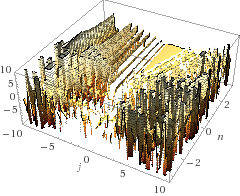
\includegraphics[width=3in]{ball_result.png}
      \caption{Probability of $r^*$ falling between the $j$th and $j+1$st largest values in the sequence $\{r_i\}_{i=1}^n$}
    \end{figure}
  \end{proof}

  \subsection{Convergence in Number of Re-encodings}

  Although DCS and RTOPE are not structurally expectation equivalent, we can examien other properties between these two schemes. In particular, we can show that as $n \to \infty$, if $R_{DCS} / R_{RTOPE} = c$ for some constant $c$ where $R_{i}$ is the number of repetitions for scheme $i$, then the number of re-encodings in DCS and RTOPE will converge to the same number.

  \begin{theorem}
    As $n \to \infty$, if $R_{DCS} / R_{RTOPE} = c$ for some constant $c$, then the number of re-econdings in DCS and RTOPE will converge to the same number.
  \end{theorem}
  \begin{proof}
  \end{proof}

  

\end{document}
